\documentclass[12pt]{article}
\usepackage[top=1cm, bottom=3cm, right=2cm, left=2cm]{geometry}
\usepackage{amsfonts, amssymb, amsmath, hyperref}
\usepackage{graphicx}
\usepackage[T1, T2A]{fontenc}% T2A for Cyrillic font encoding
\usepackage[english, russian]{babel}
\usepackage[justification=centering]{caption}
\usepackage{wrapfig,lipsum,booktabs}
\usepackage{placeins}
\usepackage{subcaption}
\usepackage{multirow}
\usepackage{indentfirst}
% \usepackage{lmodern}
% \usepackage{siunitx}

\begin{document}
\title{\textbf{Лабораторная работа 4.7.3}\\ [2pt]{Изучение поляризованного света}}
\date{\today}
\author{Татаурова Юлия, Павлов Матвей}

\begin{document}
\maketitle

\textbf{Цель работы:} Ознакомление с методами получения и анализа поляризованного света.

\textbf{Оборудование:} Оптическая скамья с осветителем; зеленый светофильтр; два поляроида; черное зеркало; полированная эбонитовая пластинка; стопа стеклянных пластинок; слюдяные пластинки разной толщины; пластинки в $ 1/4 $ и $ 1/2 $ длины волны; пластинка в одну длину волны для зеленого света (пластинка чувствительного оттенка).

\section*{Ход работы}

\subsection*{Определение разрешённых направлений поляроидов}
\begin{figure}[h]
    \centering
	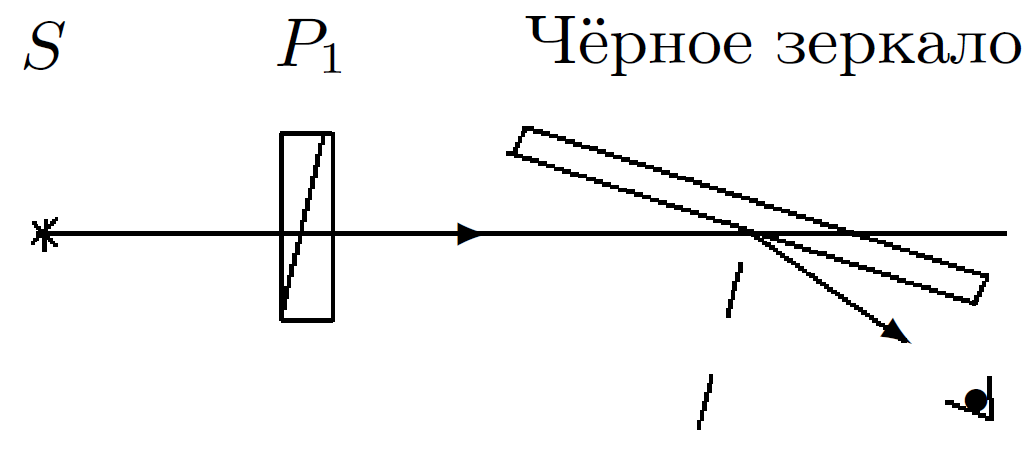
\includegraphics[width=0.5\linewidth]{images/Screenshot_1.png}
	\caption{Определение разрешённых направлений поляроида.}
	\label{pic:1}
\end{figure}
Разместим на оптической скамье осветитель $ S $, поляроид $ P_1 $ (горизонтальное направление, лимб $-10^\circ$) и чёрное зеркало. Вращая $ P_1 $, минимизируем яркость отражённого пятна, затем, поворачивая зеркало, снова уменьшим интенсивность.  

Заменим зеркало вторым поляроидом $ P_2 $, скрестим их. Разрешённое направление $ P_2 $ — вертикальное, на лимбе $ 75^\circ $.

\subsection*{Определение показателя преломления эбонита}
Заменим чёрное зеркало эбонитовой пластиной с круговой шкалой. Повернём её перпендикулярно лучу и совместим отражённое пятно с отверстием осветителя.  

Установим $ P_1 $ горизонтально и найдём угол минимальной интенсивности отражённого луча: $ 56^\circ \pm 5^\circ $. Повторим с фильтром $ F $ — результат тот же.
\\\\
По углу Брюстера рассчитаем показатель преломления эбонита.
\begin{equation}\label{eq:1}
	n = \tg 56^{\circ} = 1,5 \pm 0,3
\end{equation}

\subsection*{Исследование стопы}
\begin{figure}[h]
    \centering
	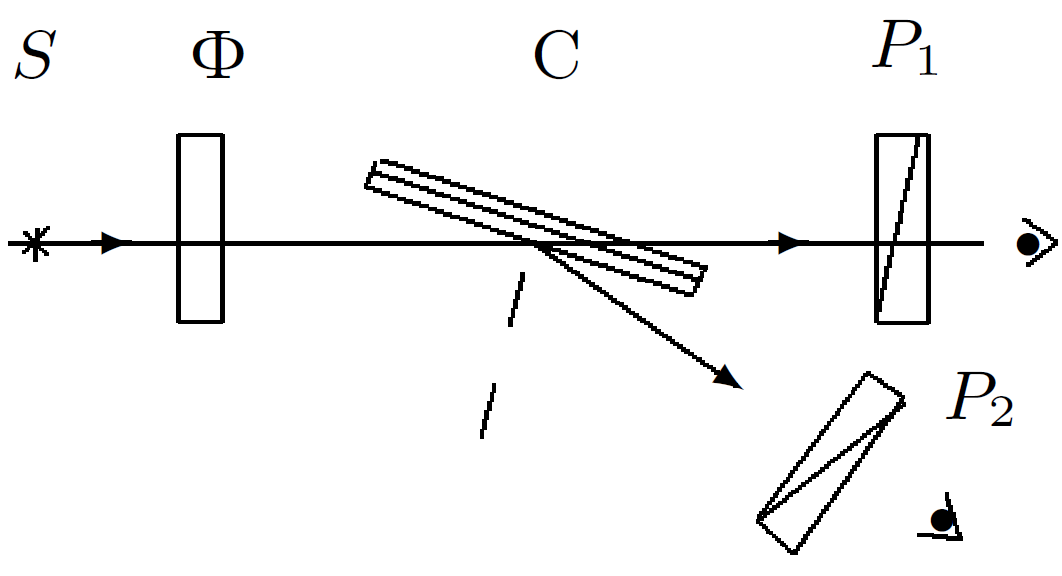
\includegraphics[width=0.5\linewidth]{images/Screenshot_2.png}
	\caption{Исследование стопы.}
	\label{pic:2}
\end{figure}

Заменим эбонитовое зеркало стопой стеклянных пластинок, настроив угол падения на угол Брюстера. Осветим её неполяризованным светом, через поляроиды определим ориентацию вектора $ \mathbf{E} $: преломлённые лучи \underline{горизонтальные}, отражённые \underline{вертикальные}.


\subsection*{Определение главных плоскостей двоякопреломляющих пластин}
\begin{figure}[h]
\centering
	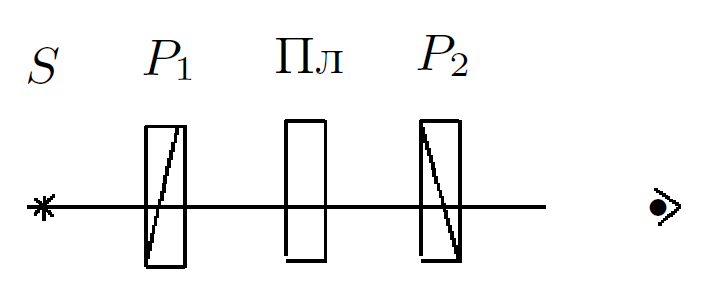
\includegraphics[width=0.5\linewidth]{images/Screenshot_3.png}
	\caption{Определение главных направлений в пластинках.}
	\label{pic:3}
\end{figure}

Между скрещёнными поляроидами $ P_1 $ и $ P_2 $ поместим кристаллическую пластинку. Вращая её, наблюдаем чередование минимумов и максимумов через $ 45^\circ $. Главные плоскости пластин совпадают с разрешёнными направлениями поляроидов при максимальной интенсивности.  

Максимумы: Первая пластинка: $ \alpha_0 = 28^\circ $; Вторая пластинка: $ \alpha_0 = 6^\circ $.

\subsection*{Выделение пластин $ \lambda / 2 $ и $ \lambda / 4 $}
Добавим к схеме зелёный фильтр, установим первый поляроид горизонтально, а главные направления пластинки — под углом $ 45^\circ $.  

\begin{table}[h]
    \centering
    \renewcommand{\arrayrulewidth}{0pt}
    \begin{tabular}{|c|c|c|}
        \hline
        \textbf{Пластинка} & \textbf{Цвет после поворота} & \textbf{Вывод} \\  
        \hline \hline
        $ \lambda / 2 $ & Фиолетовый, тускнеет & Линейная поляризация \\  
        \hline
        $ \lambda / 4 $ & Зелёный, не тускнеет & Круговая поляризация \\  
        \hline
    \end{tabular}
    
\end{table}

\subsection*{Быстрая и медленная оси $ \lambda / 4 $}

Поставим между скрещёнными поляроидами пластинку чувствительного оттенка в виде стрелки. Убедимся, что эта пластинка не меняет поляризацию зелёного света. После удаления зелёного фильтра стрелка становится пурпурной. Это объясняется тем, что зелёная компонента линейно поляризованного света при прохождении пластинки не меняет поляризацию и задерживается вторым поляроидом. 

\begin{figure}[h!]
    \centering
	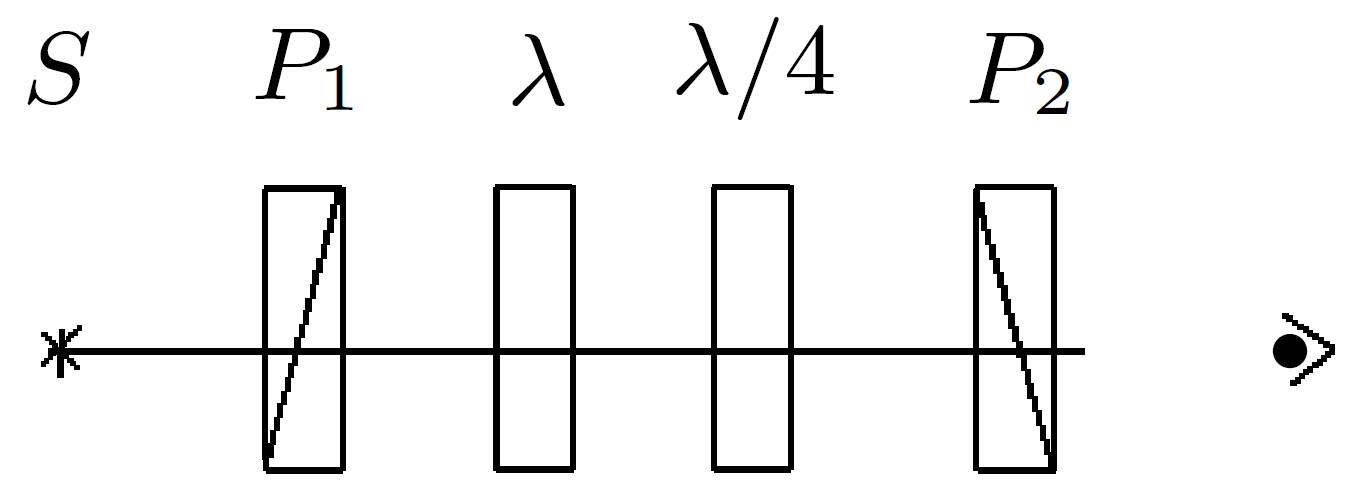
\includegraphics[width=0.5\linewidth]{images/Screenshot_4.png}
	\caption{Определение направлений большей и меньшей скорости}
	\label{pic:4}
\end{figure}

Добавим пластинку $ \lambda / 4 $ (рис. 4), главные направления которой совпадают с главными направлениями пластинки $ \lambda $ и ориентированы под углом $ 45^\circ $ к разрешённым направлениям скрещённых поляроидов.  

При повороте рейтера со стрелкой на 180° вокруг вертикальной оси цвет стрелки меняется с зелёно-голубого на оранжево-жёлтый. В первом случае у нас «быстрая» ось (они совпадают), во втором — «медленная».

\subsection*{Интерференция поляризованных лучей}



Расположим между скрещёнными поляроидами мозаичную слюдяную пластинку, состоящую из четырёх полосок разной оптической толщины, расположенных по сторонам квадрата (две полоски «толщиной» $ \lambda / 4 $ и но одной — $ \lambda / 2 $ и $ 3 \lambda / 4 $). В центре слюды нет. Главные направления пластинок параллельны сторонам квадрата.  

При вращении пластинки изменяется \textbf{интенсивность} света.

При вращении второго поляроида изменяется \textbf{цвет}.

\subsection*{Эллиптически поляризованная волна}

\begin{figure}[h]
	\center{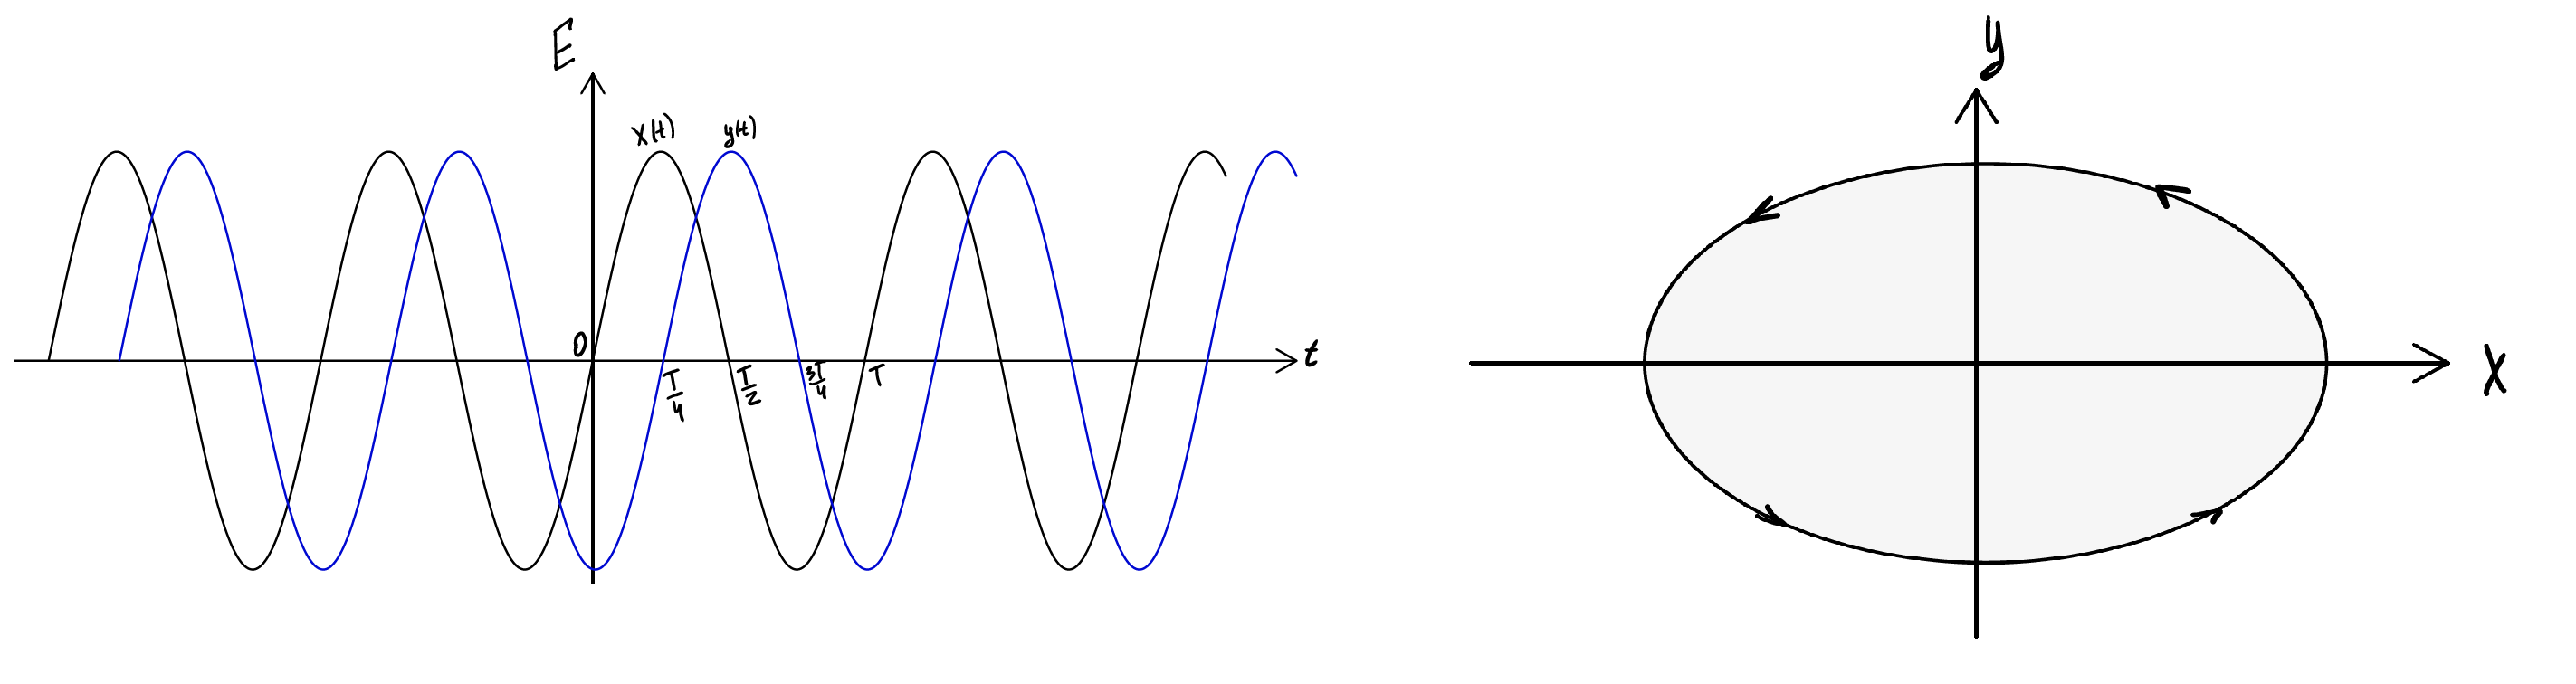
\includegraphics[width=\linewidth]{images/pics.png}}
	\caption{\centering Эллипс поляризации и графики синусоид.}
	\label{pic:5}
\end{figure}

Сначала устанавливаем зелёный фильтр, а за ним между скрещёнными поляроидами --- пластинку произвольной толщины $ (\lambda / 4) $. Получаем эллиптически поляризованный свет. Для этого поворачиваем первый поляроид под углом $ 10^\circ $–$ 20^\circ $ к горизонтали так, чтобы вектор \textbf{E} падающего на пластинку света располагался в первом квадранте. Второй поляроид устанавливаем вертикально. Вращая пластинку, определяем минимальную интенсивность света после второго поляроида. Вращая второй поляроид, убеждаемся, что свет действительно эллиптически поляризован, а не линейно. Таким образом, получаем эллипс поляризации с вертикально ориентированной малой осью.

\section{Вывод}
Таким образом, в ходе работы были получены следующие результаты:
\begin{itemize}
\item Определены разрешённые направления поряроидов --- для первого поляроида разрешённое направление горизонтальное, на лимбе $-10^{\circ}$, для второго поляроида --- вертикальная волна, на лимбе $75^{\circ}$;
\item Был определен показатель преломления эбонита по углу Брюстера:
\begin{equation*}
    n = \tg{56^{\circ}} = 1,5 \pm 0,6
\end{equation*}
Полученный результат в пределах погрешности совпадает с табличным $n = 1,6$;
\item Получили, что в стопе стеклянных пластинок преломленные лучи горизонтальные, а отраженные --- вертикальные;
\item Для двоякопреломляющих пластин определены главные направления --- минимумы и
максимумы интенсивности чередуются через $45^{\circ}$, главные плоскости пластин совпадают с разрешенными направлениями поляроидов при максимальной интенсивности. Максимумы: для первой $\alpha_0 = 28^{\circ}$, для второй $\alpha_0 = 6^{\circ}$;
\item Выяснили, что из двух имеющихся пластинок первая из них --- пластинка $\lambda/2$, а вторая --- $\lambda/4$;
\item «Быстрая» ось пластинки $\lambda/4$ совпадает с «быстрой» осью пластинки $\lambda$ и ориентирована под углом $45^{\circ}$ к разрешенным направлениям скрещенных поляроидов. При повороте рейтера со стрелкой на $180^{\circ}$ вокруг вертикальной оси получаем медленную ось.
\item При изучении интерференции поляризованных лучей было получено, что при вращении пластинки в отдельном квадратике изменяется интенсивность, а при вращении второго поляроида --- изменяется цвет;
\item Было определено направление вращения светового вектора в эллиптически поляризованной волне после пластинки $\lambda/4$: оно компенсирует разность фаз со второй пластинкой, «быстрая» и «медленная» оси которой известны. Таким образом, эллипс первой пластинки вращается в противоположную сторону.
\end{itemize}

\end{document}
